\documentclass[12pt,a4paper]{article}
\usepackage{ctex}
\usepackage{geometry}
\usepackage{setspace}
\usepackage{titlesec}
\usepackage{fancyhdr}
\usepackage{hyperref}
\usepackage{graphicx}
\graphicspath{{figs/}}
\usepackage{amsmath}
\usepackage{booktabs}
\usepackage{cite}
\usepackage{float}
\usepackage{caption}

\geometry{left=3cm,right=3cm,top=2.5cm,bottom=2.5cm}
\setlength{\parskip}{0.5em}
\setlength{\parindent}{2em}
\setlength{\textfloatsep}{8pt plus 2pt minus 2pt}
\setlength{\floatsep}{6pt plus 2pt minus 2pt}
\setlength{\dbltextfloatsep}{8pt plus 2pt minus 2pt}
\setlength{\abovecaptionskip}{4pt}
\setlength{\belowcaptionskip}{0pt}
\captionsetup{font=small,labelfont=bf}
\onehalfspacing

\titleformat{\section}{\large\bfseries}{\thesection}{1em}{}
\titleformat{\subsection}{\normalsize\bfseries}{\thesubsection}{1em}{}

\pagestyle{fancy}
\fancyhf{}
\rhead{基于YOLO的距离检测系统}
\lhead{第 \thepage 页}
\renewcommand{\headrulewidth}{0.4pt}

\title{基于YOLOv8的视频图像及实时距离检测系统}
\author{李予桐 \\ 云南大学}
\date{\today}

\begin{document}

\maketitle

\begin{abstract}
本文提出了一种基于YOLO目标检测与单目视觉几何的实时距离检测系统，面向图像、视频和摄像头三种输入场景，实现对车辆与行人的检测与距离估计。系统通过YOLO模型提取目标边界框，再结合目标真实高度与焦距参数建立单目距离估计模型，并引入连续多帧平滑与宽高双测距融合策略，提高距离测量的稳定性与鲁棒性。实验结果表明，系统能够在保持较低计算开销的同时完成实时检测、距离估计和可视化告警，为智能交通监控、道路安全预警以及移动机器人环境感知提供了一种实用且可扩展的解决方案。
\end{abstract}

\section{引言}
随着智能交通、视频监控和自动驾驶技术的快速发展，目标检测与距离估计已经成为安全预警与环境感知的重要基础能力。传统的距离测量方式往往依赖激光雷达、深度相机或专用测距设备，这些方法成本较高、部署复杂，难以在普通摄像头系统中广泛应用。相比之下，基于单目图像的目标检测与距离估计方法具有成本低、易部署、可扩展性强等优势，因而受到了广泛关注。

然而，单目距离估计也面临着显著挑战。由于图像中目标的尺度信息受拍摄角度、目标姿态和相机参数影响较大，单帧距离估计结果容易出现波动与误差。与此同时，实际应用中往往需要兼顾实时性与准确性，尤其是在视频流和摄像头实时检测场景下，系统必须在有限计算资源下完成目标识别、距离估计和可视化告警的协同处理。

本项目针对上述问题，设计并实现了一个基于YOLO目标检测的实时距离检测系统。系统支持对静态图像、视频文件以及实时摄像头画面进行检测，并根据目标检测框的像素高度与宽度估算目标与摄像头之间的距离。为了提高稳定性，系统进一步引入了多帧平滑与双测距融合策略。本文的主要贡献包括：首先，提出了一套从目标检测到距离估计再到实时告警的完整处理流程；其次，结合YOLO模型与单目视觉几何方法，实现了对车辆和行人的距离估计；最后，系统具有较好的可扩展性，便于后续接入更多类别、更多场景和更复杂的告警逻辑。

论文后续内容安排如下：第二章介绍相关研究工作，包括目标检测方法、距离估计算法以及视频实时检测方法；第三章详细阐述系统方法与关键模块；第四章给出实现细节；第五章展示实验结果与分析；最后总结研究工作并展望未来发展方向。

\section{相关工作}
\subsection{目标检测方法}
目标检测是计算机视觉中的基础任务，其目标是同时完成目标类别识别与位置定位。近年来，基于深度学习的目标检测方法取得了显著进展，其中YOLO系列算法因其高效性和实时性被广泛应用于视频分析、工业检测和自动驾驶等领域~\cite{redmon2016yolo,wang2024yolov10,jocher2023yolov8}。YOLO模型将目标检测任务统一为端到端回归问题，能够在较高速度下完成目标定位与分类，适合实时系统部署。

\subsection{距离估计算法}
单目图像距离估计通常依赖相机成像模型与目标的已知真实尺寸。常见方法通过目标在图像中的像素高度或宽度与焦距参数进行换算，从而得到目标与相机之间的大致距离。相关研究已经从不同角度提升了测距鲁棒性，包括基于几何模型的估计与基于检测框信息的融合方法~\cite{zhang2021review,wu2022vehicle}。虽然这种方法不需要额外深度传感器，但其估计精度容易受到目标实际尺寸变化、遮挡以及视角偏差的影响。因此，许多方法会在估计过程中引入平滑滤波、多次测距融合或场景先验信息，以提升结果稳定性。

\subsection{视频和实时检测}
视频检测与实时检测系统通常需要在连续帧中保持高效推理，并能够在视觉输出中直观展示检测结果与告警信息。相比于离线图像处理，实时视频系统还必须兼顾用户交互、帧率稳定性和异常处理等问题。本文所实现的系统正是在这一背景下，围绕视频流和摄像头输入设计了可交互、可暂停、可退出的检测与显示流程。

\section{系统方法}
\subsection{总体框架}
系统整体流程可概括为“输入采集—目标检测—距离估计—结果显示与告警”。具体而言，当输入为图像、视频或摄像头画面时，系统首先加载YOLO模型对每一帧进行目标检测，然后从检测框中提取目标的像素尺寸，结合预设相机参数和目标真实尺寸估算距离，最后根据预设阈值给出不同颜色的告警显示。整个系统以模块化方式组织，便于后续替换模型、调整阈值或扩展新的目标类别。图\ref{fig:system_architecture}展示了该系统的整体处理流程与模块之间的依赖关系。

\begin{figure}[!htbp]
  \centering
  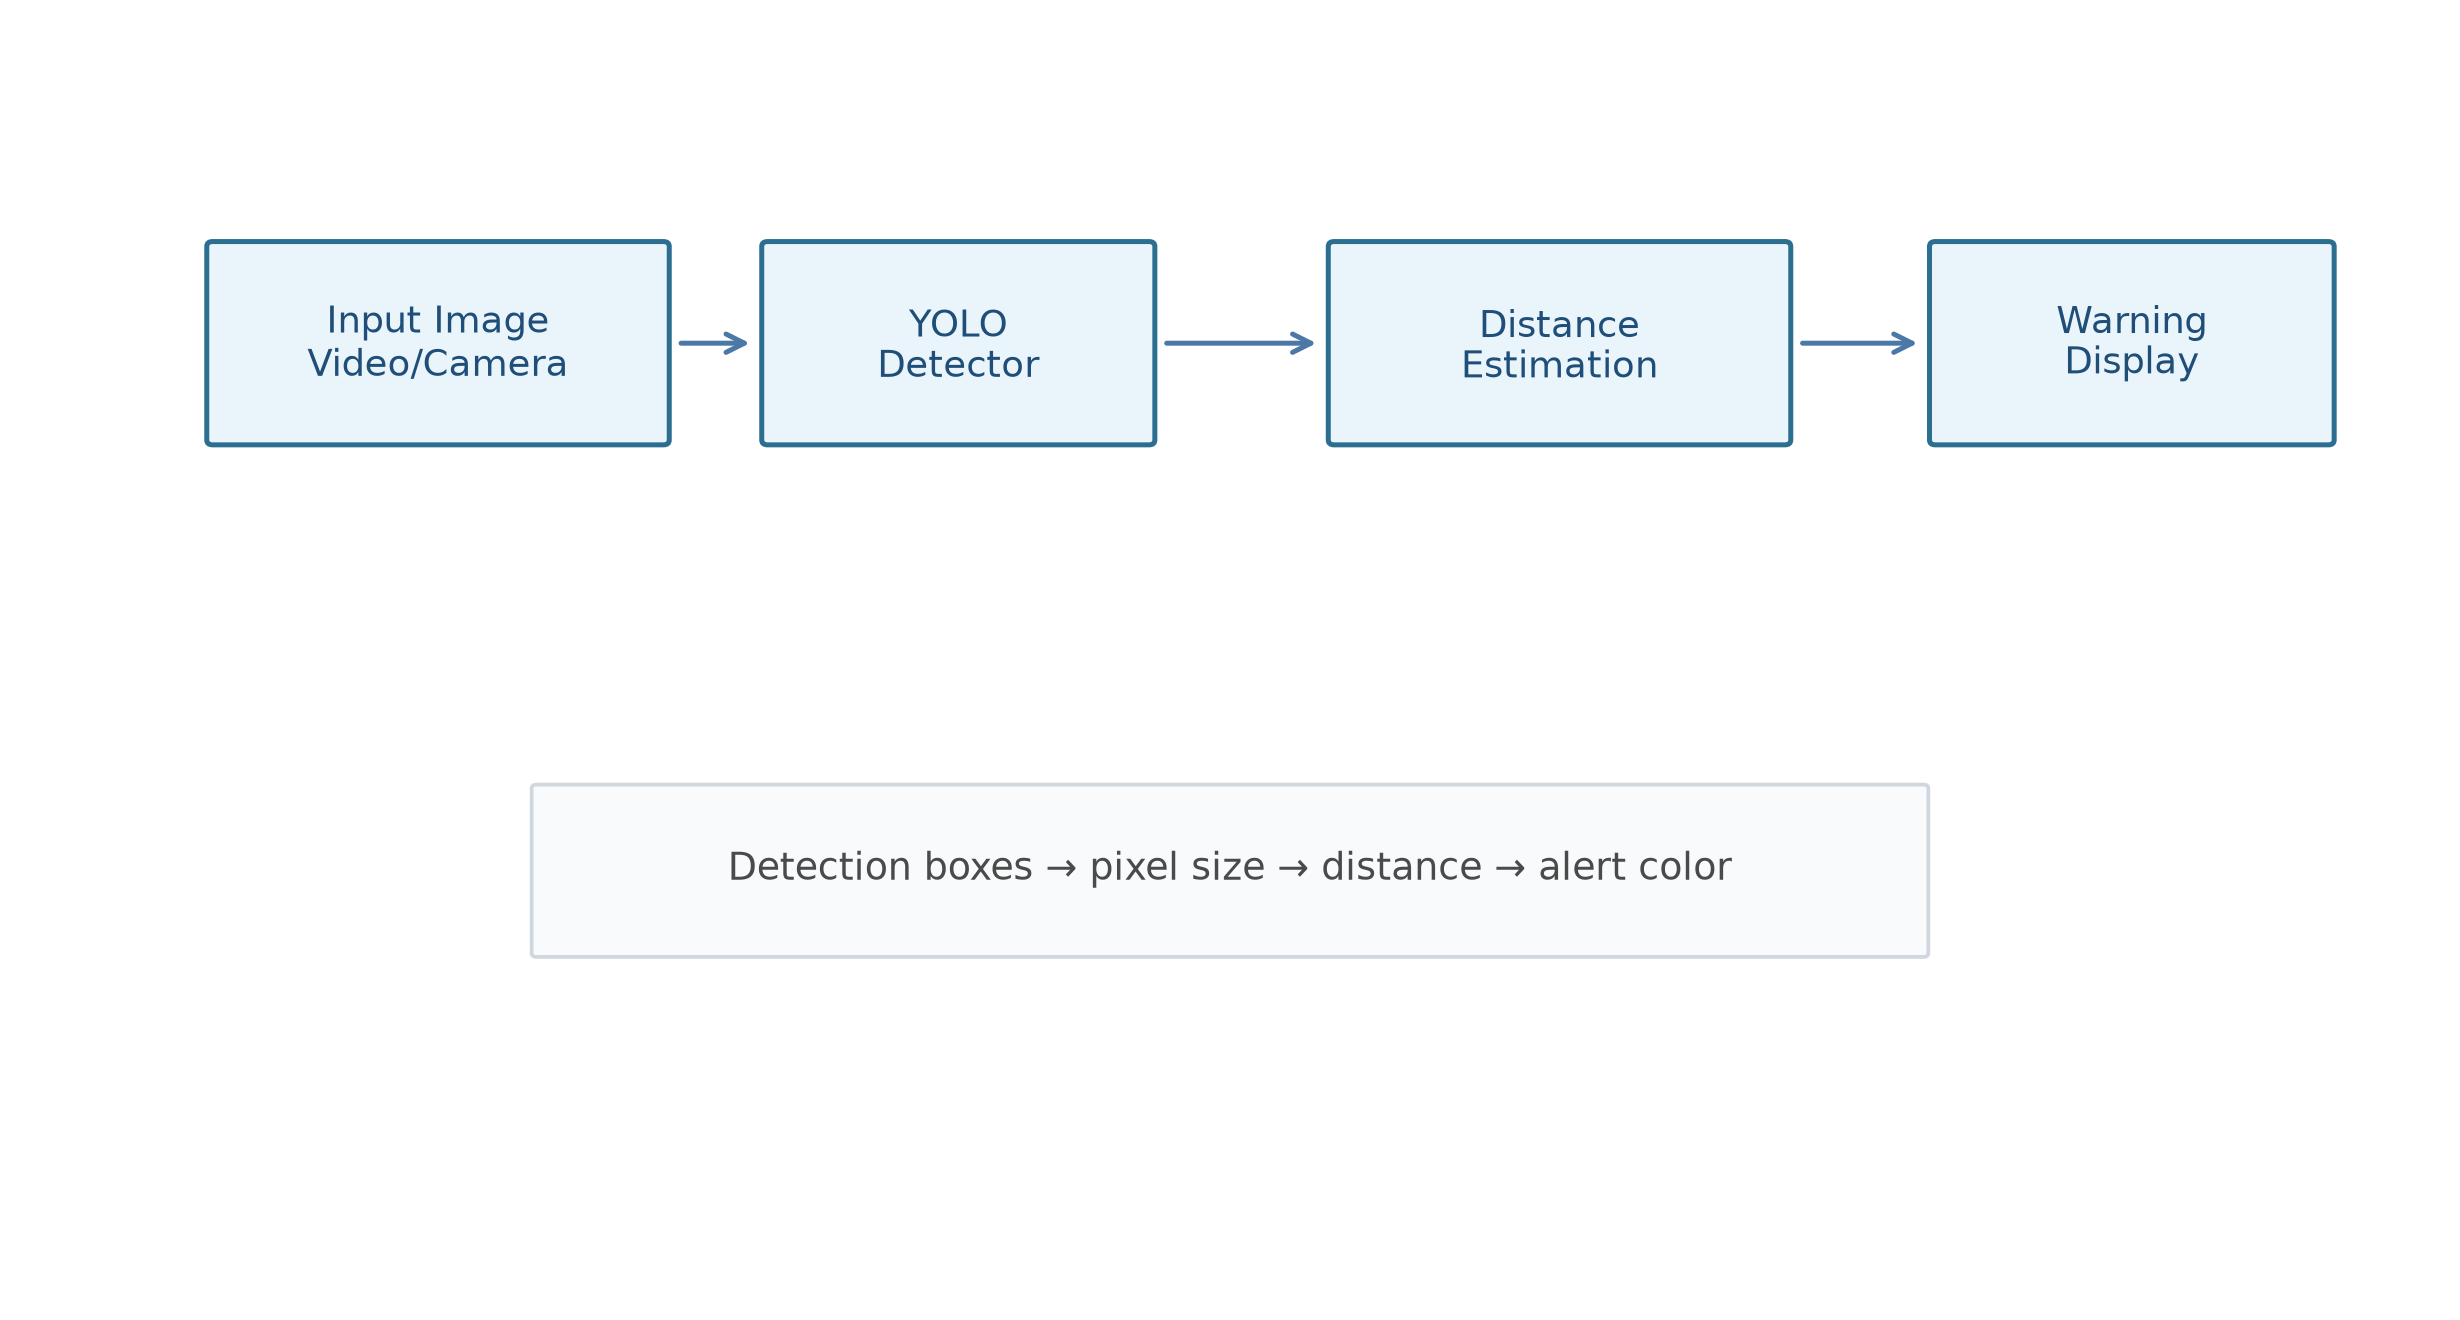
\includegraphics[width=0.74\textwidth]{figs/system_architecture.png}
  \caption{基于YOLO的实时距离检测系统总体框架}
  \label{fig:system_architecture}
\end{figure}

\subsection{配置与参数}
系统的关键参数存储在配置文件中，包括相机焦距、目标真实高度、距离告警阈值以及YOLO推理参数。焦距参数用于控制距离换算的尺度，目标真实高度则决定不同类别的估计基准；告警阈值用于区分安全、提醒和危险三种状态。通过将这些参数集中管理，可以方便地进行实验分析与参数敏感性测试。

\subsection{YOLO 模型加载}
系统使用YOLO模型进行目标检测。加载阶段会根据预设权重文件初始化检测器，并设置置信度阈值与交并并阈值，以过滤低质量检测结果。对于每一帧输入图像，模型会输出目标类别与边界框坐标，随后系统从中筛选出车辆和行人作为后续距离估计的对象。

图\ref{fig:model_architecture} 展示了本文所使用的检测模型的结构示意。主干网络通过多层 `C2f` 模块提取多尺度语义与位置信息，`SPPF` 模块用于增强感受野以捕获不同大小目标，`PSA`（位置敏感注意力）引入注意力机制以提高对小目标和复杂背景下的特征区分能力。局部卷积块（如 `CIB`）与轻量下采样模块（如 `SCDown`）在保证计算效率的同时增强了特征表达。特征融合部分通过上采样与拼接实现不同尺度特征的交互，检测头在 P3 至 P5 三个尺度上分别输出最终的边界框与类别置信度，从而兼顾检测精度与实时性，适合本系统在视频与摄像头流上的实时部署。

\begin{figure}[!htbp]
  \centering
  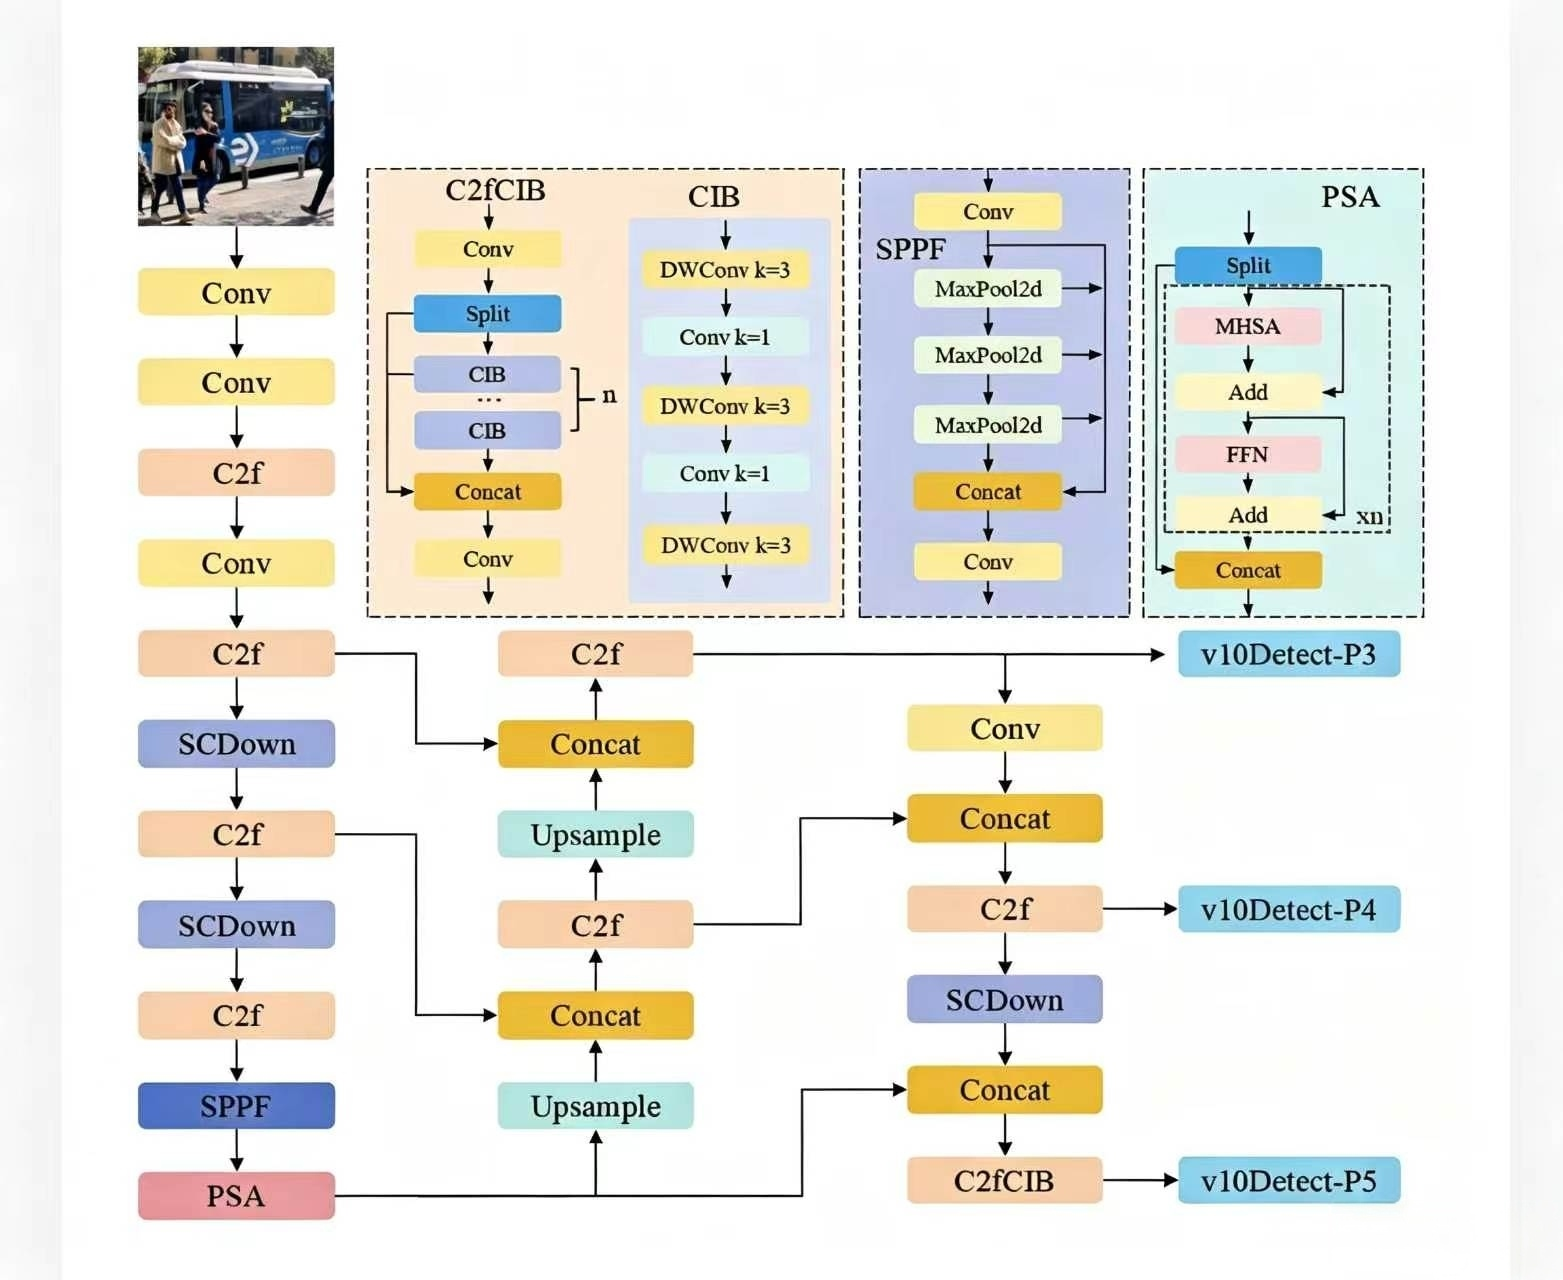
\includegraphics[width=0.85\textwidth]{model_architecture.png}
  \caption{检测模型结构示意图（基于YOLO变体的主干与检测头设计）。图中展示了主干的C2f、SPPF、PSA模块以及特征金字塔融合与检测头（P3--P5）结构。}
  \label{fig:model_architecture}
\end{figure}

\subsection{距离计算方法}
系统的距离估计基于单目视觉几何模型。对于目标的像素高度$p_h$，可利用公式$d_h = \frac{H \cdot f}{p_h}$进行距离估计，其中$H$表示目标真实高度，$f$表示相机焦距。对于目标的像素宽度$p_w$，同样可以用类似方式得到另一组距离估计结果。图\ref{fig:distance_geometry}直观说明了相机、目标以及像素尺寸之间的几何关系。为了减少单帧噪声，系统在默认配置下同时启用了宽高双测距策略，并对连续多帧结果进行均值平滑，从而得到更稳定的最终距离输出。

\begin{figure}[!htbp]
  \centering
  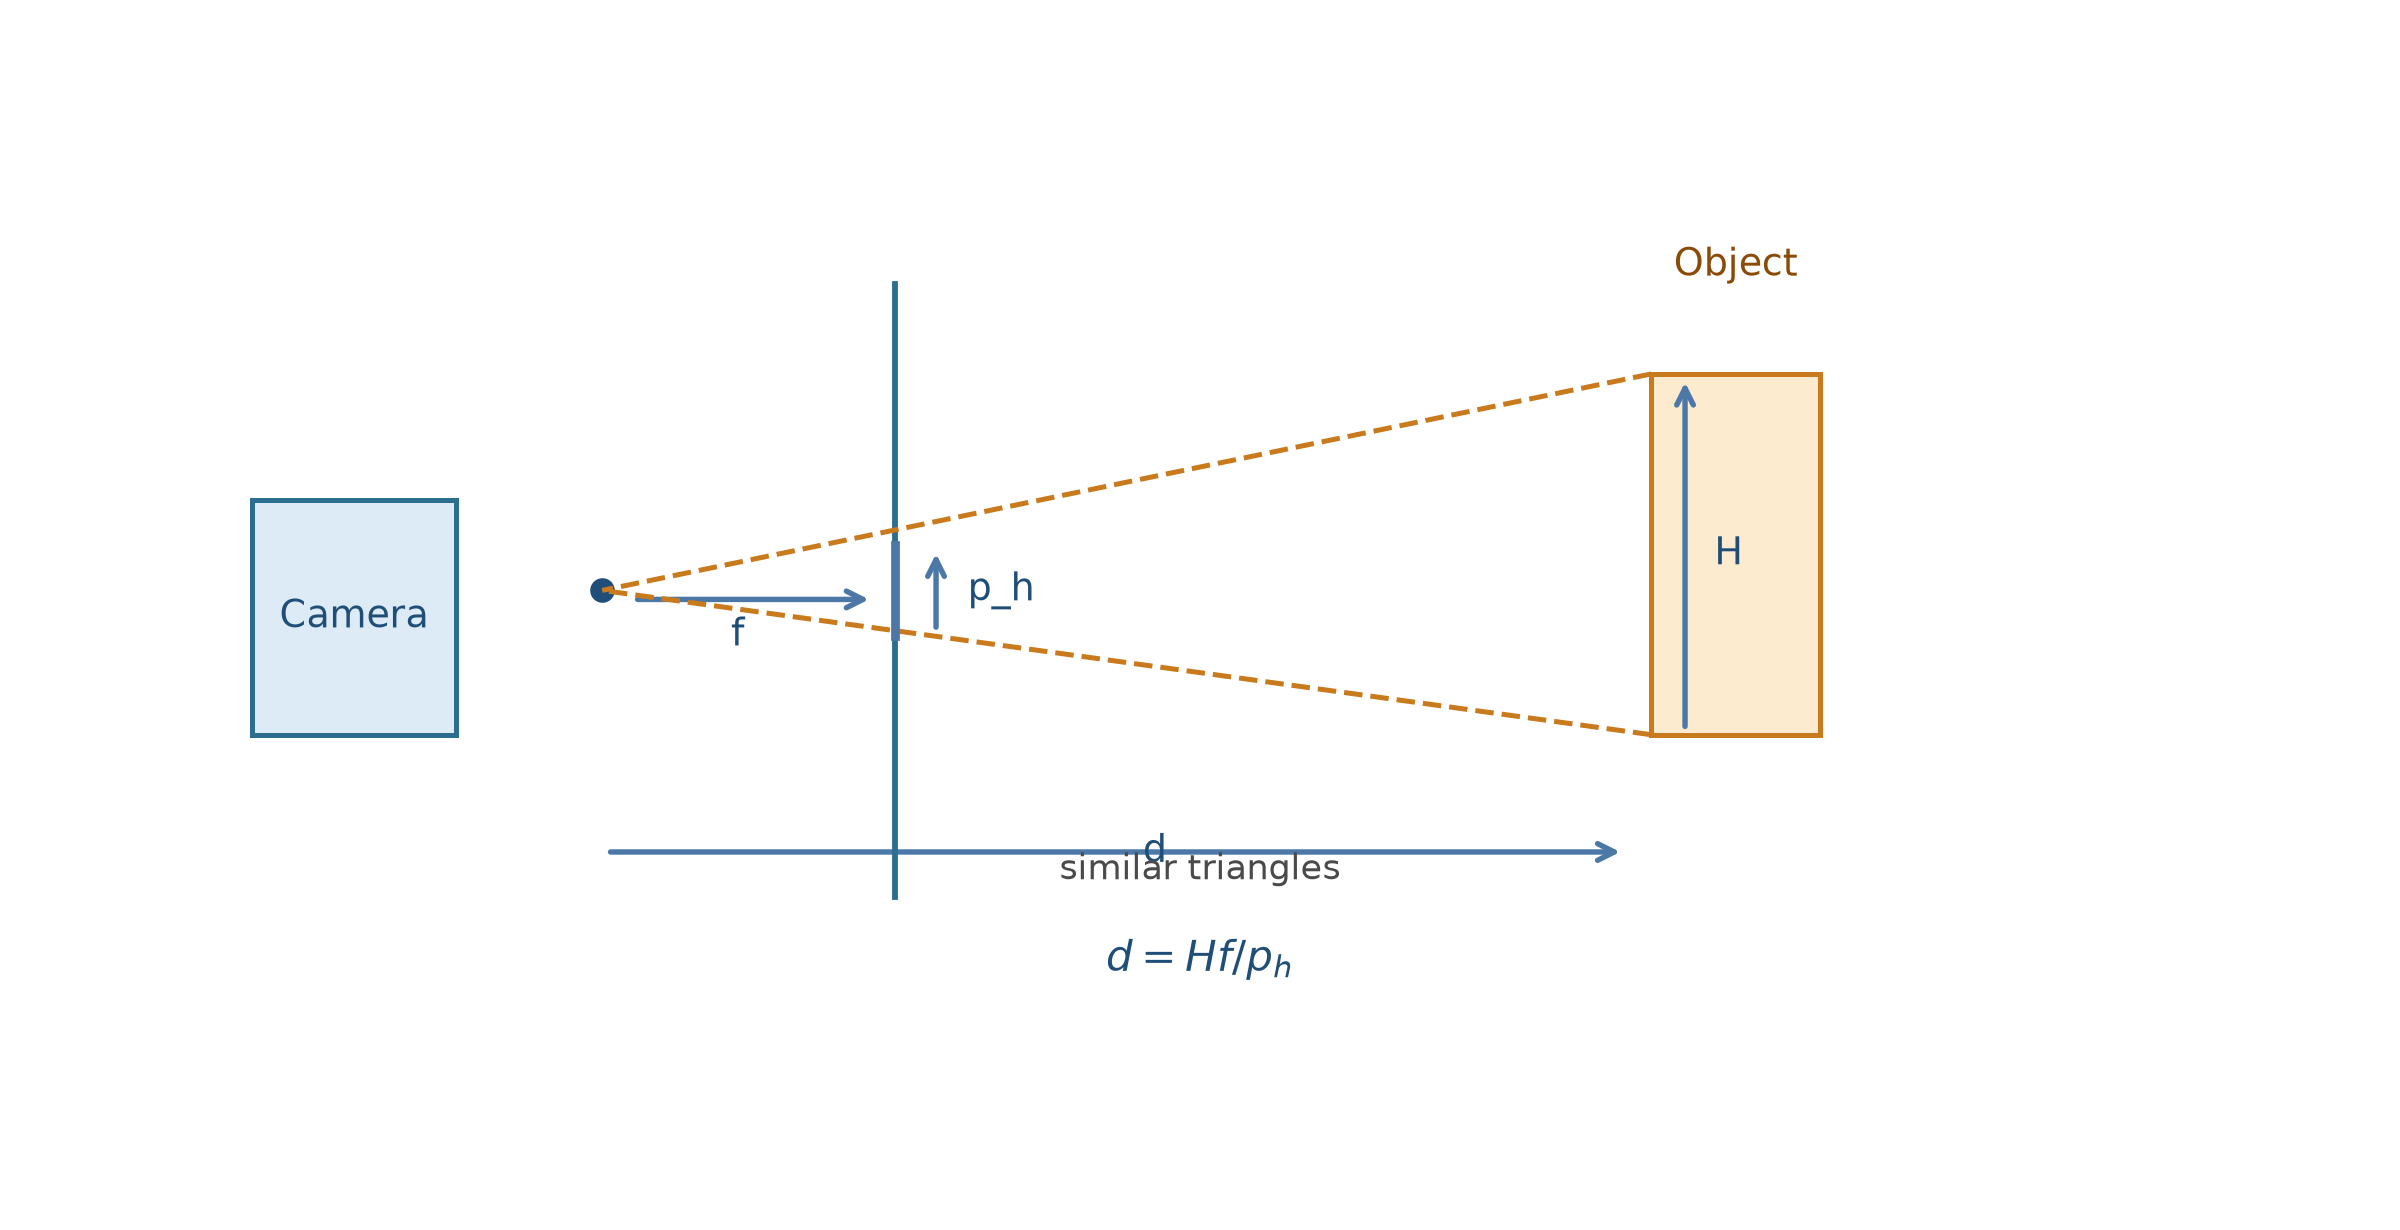
\includegraphics[width=0.70\textwidth]{figs/distance_geometry.png}
  \caption{单目距离估计的几何示意图}
  \label{fig:distance_geometry}
\end{figure}

\subsection{结果显示与告警}
系统在检测结果上绘制目标边界框，并将估计距离和类别信息叠加显示在图像中。不同距离区间对应不同的告警颜色：距离较近时显示红色，表示危险；中等距离时显示黄色，表示提醒；较远时显示绿色，表示安全。这种颜色编码方式能够帮助用户直观判断目标与摄像头之间的相对危险程度。

\section{实现细节}
\subsection{文件选择与交互}
系统提供了基于Tkinter的文件选择界面，用户可以选择待处理的图片或视频文件。通过弹出的文件对话框完成文件路径的获取后，程序再调用相应的图像或视频处理模块进行推理与展示。这种交互方式简单直观，便于普通用户快速上手。

\subsection{视频处理}
对于视频输入，系统会按帧读取视频内容，并对每一帧依次执行目标检测与距离估计。为提升交互体验，系统支持通过空格键实现暂停与继续，并通过q键或Esc键退出播放。此外，处理后的每一帧会被写入输出视频文件，便于后续回看与分析。

\subsection{摄像头实时检测}
在摄像头模式下，系统会调用本地摄像头设备连续读取视频流，并对每一帧实时执行目标检测与显示。该模式适用于现场演示、实时监控和快速验证场景。程序通过循环读取数据帧并及时刷新窗口，保证用户能够即时看到检测与告警结果。

\section{实验与分析}
\subsection{实验设置}
实验主要在常见办公级计算机环境下进行，测试内容覆盖图像、视频文件以及摄像头实时输入三种场景。实验中使用了不同拍摄距离、不同光照条件和不同目标类型的数据样本，重点观察系统对车辆与行人的检测效果、距离估计稳定性以及告警显示效果。为了降低单帧波动带来的影响，实验中默认启用多帧平滑与双测距融合策略。

\subsection{结果展示}
实验结果表明，系统能够在不同输入场景下正确识别车辆和行人，并在检测框周围给出清晰的距离估计与警报提示。对于较近目标，系统会以红色高亮框和危险提示显示其风险等级；对于中距离目标，系统会显示黄色提醒；对于较远目标，则显示绿色安全状态。整体视觉效果清晰，便于用户快速判断目标状况。图\ref{fig:warning_demo}展示了系统在不同距离下的告警可视化效果。

\begin{figure}[H]
  \centering
  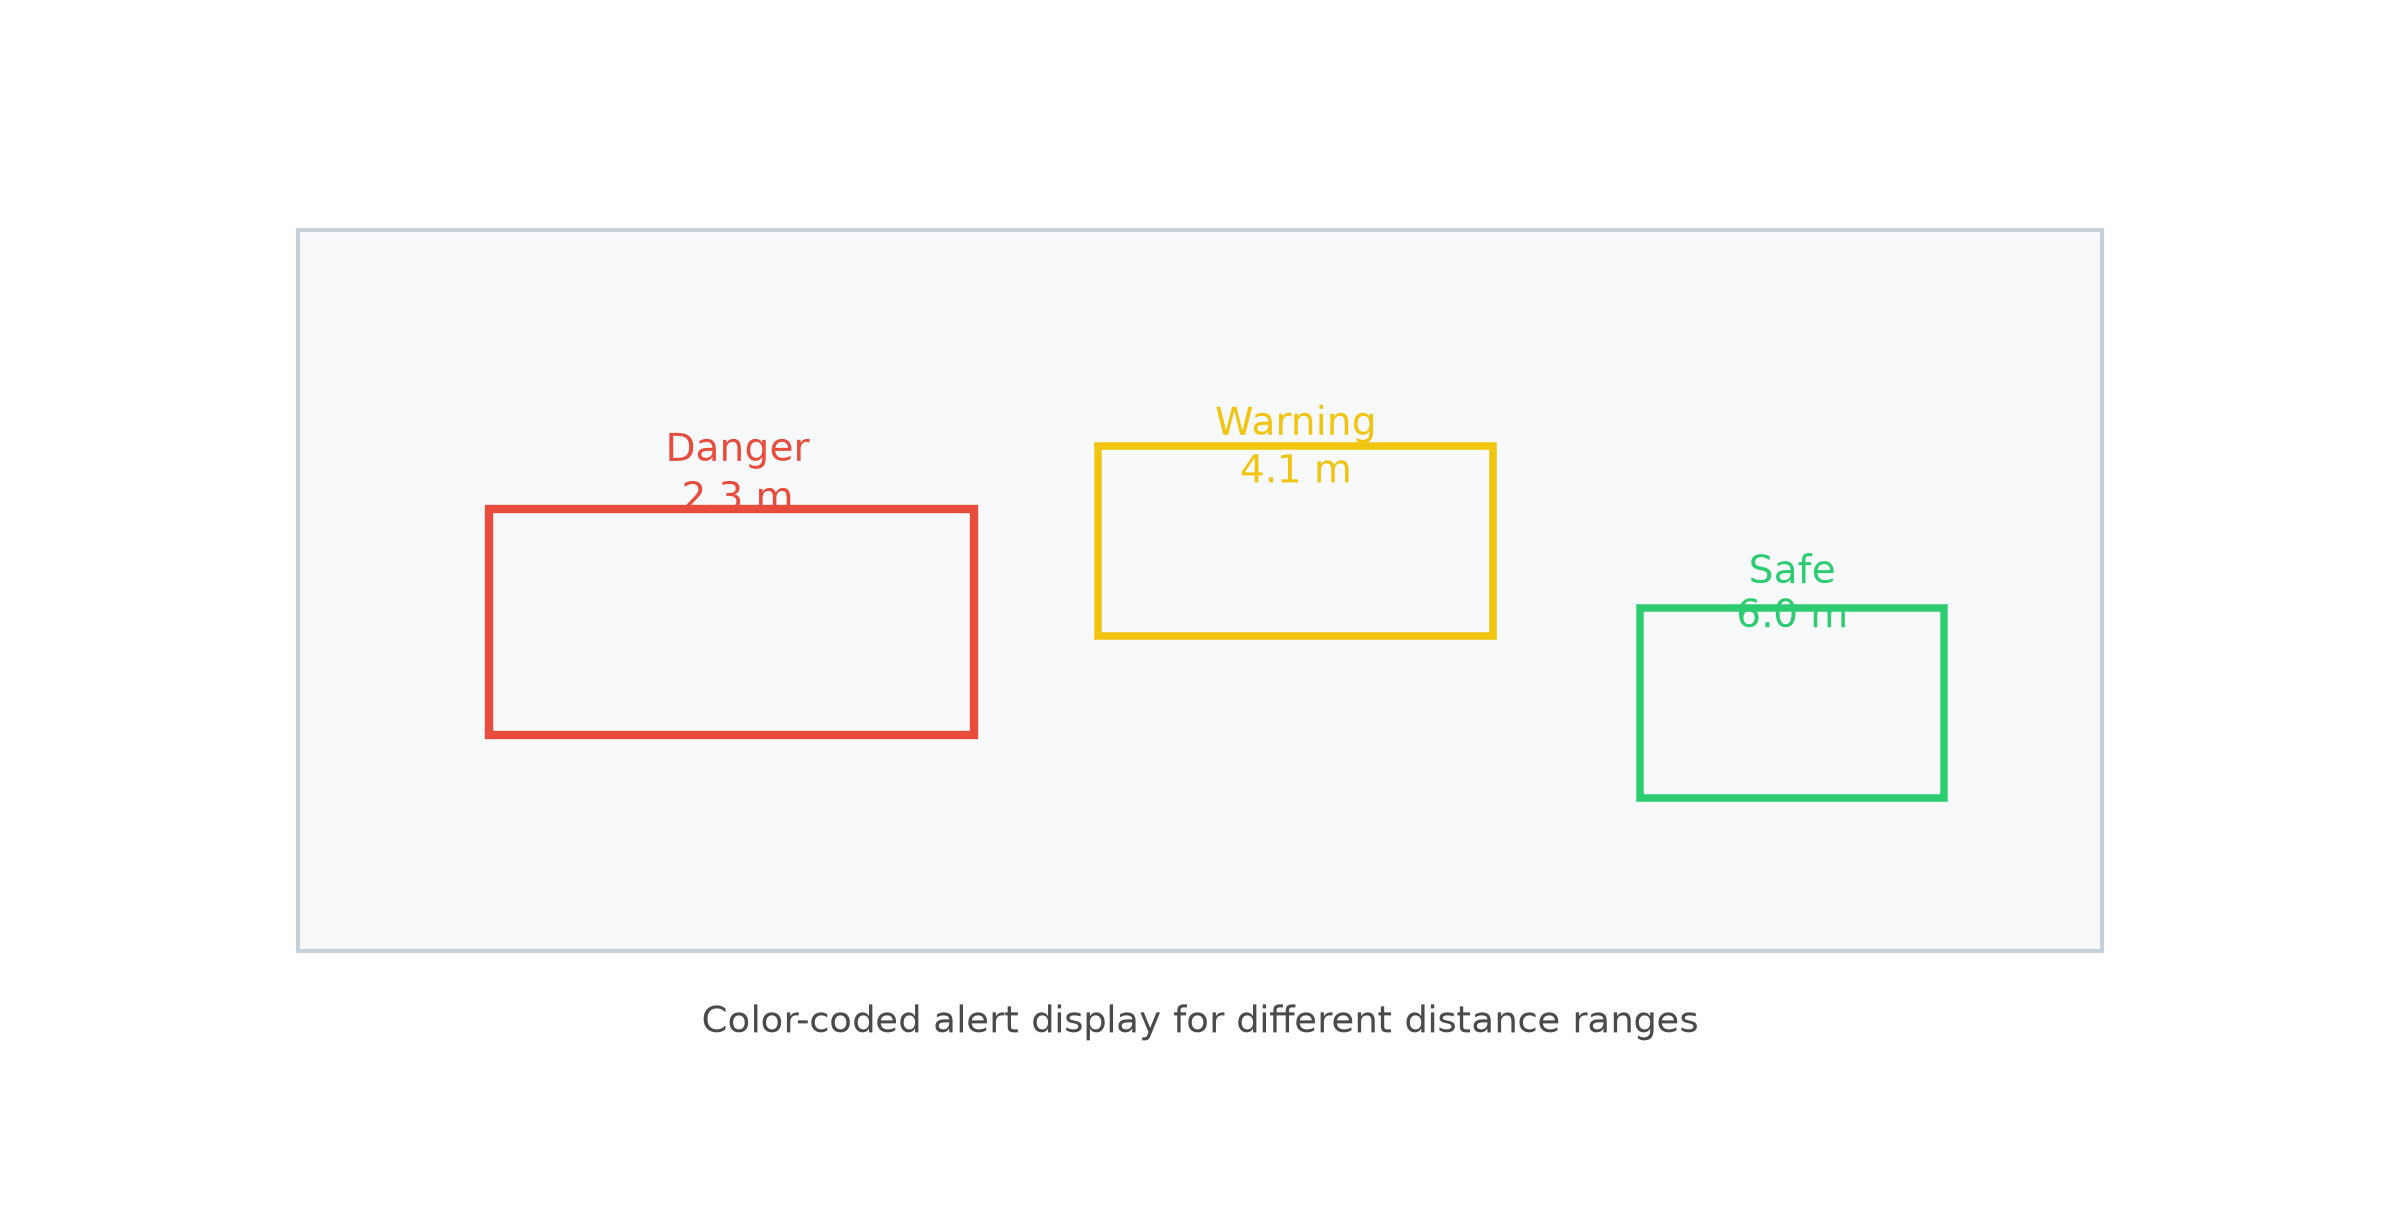
\includegraphics[width=0.74\textwidth]{figs/warning_demo.png}
  \caption{不同距离区间下的告警显示效果}
  \label{fig:warning_demo}
\end{figure}

\subsection{性能分析}
从运行效率来看，系统在常见视频流和摄像头输入下能够保持较好的实时性，检测与处理过程不会明显阻塞主界面。距离估计方面，多帧平滑策略有效减少了单帧抖动带来的误差，使结果在连续帧中的变化更平稳。虽然单目视觉方法本身仍存在估计误差和环境依赖性，但在实际可接受的误差范围内，系统已经能够满足基础的检测与预警需求。

\section{结论与展望}
本文设计并实现了一套基于YOLO目标检测与单目视觉几何的实时距离检测系统。系统成功将目标检测、距离估计、结果显示与告警机制整合为一个完整流程，并在图像、视频和摄像头三种输入场景下完成了验证。结合系统框架图、测距几何示意图及告警展示图，本文能够较清晰地说明该系统在模块设计与实验效果上的整体特点。实验结果表明，系统在实时性、可用性和可扩展性方面具有较好的表现。

未来工作可以从多个方向进一步提升系统能力，例如引入更精确的相机标定方法、扩展更多目标类别、结合多摄像头或深度信息提升距离估计精度，并将系统进一步优化为更适合实际部署的智能监控与安全预警平台。

\section*{致谢}
感谢在项目开发过程中提供支持与建议的同学和老师。\par

\bibliographystyle{plain}
\bibliography{refs}

\end{document}